%%%% This is the general thesis/project report template for most users
\documentclass[10pt,showtrims,b5paper]{rubook}
%% RU Book options (subclass of memoir)
%% 10pt:  default font -- DO NOT CHANGE
%% showtrims:  indicate where printer will cut to size
%% a4paper or b5paper:  paper stock size.
%%     If A4, show cut lines.  If b5, no cut lines.
\usepackage[]{ruthesis}
%% Options for ruthesis in []:
%%   IS Icelandic is main language, otherwise default to English

%%%%%% Packages and Macros %%%%%%%%%%%%%%%%%%%%%%%%%%%%%%%%
\usepackage{custom}
%% Commonly-used packages and macros are in custom.sty
%% Put any additional packages after this line
%% !!WARNING: The geometry package is incompatible with this template!

\usepackage{lipsum}%provides us with text for testing
%% usage: \lipsum[STARTNUM-ENDNUM]
%%%%%%%%%%%%%%%%%%%%%%%%%%%%%%%%%%%%%%%%%%%%%%%%%%%%%%%

\title{Thesis and Project Report Template for \theInstitution{}}
\author{Joseph~T.~Foley and Marcel~Kyas}
\date{2022}{5}{5}%{Year}{Month}{Day}%use numbers

%\DocumentInfo{TYPE}{ABBREVIATION}{DEGREE}{PROGRAM}{ECTS}{School/Department}
\DocumentInfo{Thesis}{M.Sc.}{Master of Science}{Mechatronics}{30}{Department of Engineering}
\DocumentDescription{\theDocumentType{} of \theECTS{} ECTS credits
         submitted to the \theSchool{} at \theInstitution{} in partial fulfillment
         of the requirements for the degree of \theDegreeLong}
% Change this if you need a custom title or if it needs to be in Icelandic

%% PhD only have Thesis Committee with roles.  Examiner is part of committee.
\SupervisorHeading{Thesis Committee}
\Supervisors{
  \personinfo{Superior A. Teacher}{Supervisor}{Professor}{Reykjavik University}{Iceland}
  \personinfo{Helpful A. Teacher}{Co-advisor}{Assistant Professor}{University of Iceland}{Iceland}
  \personinfo{Tough E. Questions}{Examiner}{Associate Professor}{Massachusetts Institute of Technology}{USA}
}

\begin{document}
%% TODO: get the official cover graphic and have the system fill in the fields for you
\maketitle{}
\copyrightpage{}
% If this is a PhD, register for an ISSN and ISBN, then:
% \copyrightpage{ISSN xxxx-yyyy\\ISBN 978-xxxxxxxxxx\\}
%\signaturepage{} %Generally only for Print copies

%\begin{dedications}% Optional
%  I dedicate this to my spouse/child/pet/power animal.
%\end{dedications}

\enableindents{}% turn on/off paragraph indents
% RUM: "Acknowledgements (optional)"%start numbering

\clearpage{}
\tableofcontents{}\clearpage
\listoffigures{}\clearpage
\listoftables{}\clearpage

%% A list of abbreviations is an example of a special list
%% Other lists may be added, such as lists of algorithms, symbols, theorems, etc.
%% IN CS PhD, this is sometimes centered.
\chapter*{List of Symbols}%%RUM: Not mentioned
%% This list demonstrates the "siunitx" package capabilities
\begin{tabular}{lll}
Symbol &Description &Value/Units\\
$E$ &Energy &\si{\joule}\\ %New function:  \unit{} in Livetex 2021
$m$ &Mass &\si{\gram}\\ %New function:  \unit{} in Livetex 2021
$c$ &Speed of Light &\SI{2.99E9}{\meter\per\square\second}\\ %New function:  \qty{} in Livetex 2021
\end{tabular}

\begin{abstract}
  The goal of this template is to produce electronic output to be uploaded to Skemman that can be later printed out and bound into a professional looking textbook that fits on standard library shelves.
  It is important to note that A4 paper when bound requires taller shelf spacing, so the B5 paper format was chosen instead.
  When binding a book, the edges that face outward need to be very smooth to reduce contamination and dust from entering the book when it sits on a shelf; this is why traditionally a larger paper size is cut down to the book size.
  If your print house expects the stock to be A4, then make sure the rubook has the ``a4paper'' option.
  If they prefer to deal with preparation themselves from a B5 pdf, then the default ``b5paper'' option is correct.
  
  
  The abstract goes here in English or Icelandic.
  It should be a fairly short summary of the entire document.
  If you switch to Icelandic mode (IS option to ruthesis) then abstract will become \'{U}tdr\'{a}ttur

  Keywords / Efnisord:  Keywords, separated, by, commas
\end{abstract}


% RUM: "Acknowledgements (optional)"
\chapter*{Acknowledgments} 
\begin{quotation}
So long, and thanks for all the fish.
\end{quotation}\sourceatright{Douglas Adams\cite{adams84fish}}
\vspace{\baselineskip}

This work was funded by \the\year~RANNIS grant ``Survey of man-eating Minke whales'' 1415550.
Additional equipment was generously donated by the Icelandic Tourism Board.

{\em Acknowledgements are optional; comment this chapter out if they are absent
  Note that it is important to acknowledge any funding that helped in the work\/}
%\/ is italic correction at the end of \em and italics
\clearpage{}

\mainmatter{}
\aliaspagestyle{chapter}{empty}
% Don't put page numbers on the chapter changes

%% If you would like to separate chapters into different files, use
%% \include{chapterfile}
%% WARNING: Make sure that all of these files (and any new ones)
%% are UTF-8 otherwise you will get weird encoding errors.
\part{Getting Started} % Parts optional but useful in longer documents
\chapter{Instructions}
\textbf{Is this the right template for you?}
If you are not a Reykjavik University student, this is probably not for you.
For everyone else, please read the instructions before getting started.
It is likely to save you a lot of frustration and errors.
% Uncomment the lines with a single % if you wish to process the document separately
% \documentclass[12pt,a4paper,titlepage,draft]{memoir}
% \usepackage[]{ruthesis}
% \usepackage{custom}
% \graphicspath{{graphics/}{Graphics/}{./}}
% \author{Joseph~T.~Foley\formatemail{foley}}  % My name, for the titlepage
% \title{Project Report and Thesis Preparation Instructions}  % The title, for the titlepage
% \renewcommand{\maketitlehookc}{}% Skip the degree details
% \renewcommand{\maketitlehookd}{}% Skip the supervisor details
% \usepackage[hidelinks]{hyperref} % must be last package loaded!

%% Macros for filling in commonly changed items
\newcommand{\TIheadofgrad}{Slawomir Koziel~\formatemail{slawomir} or TD Person}
\newcommand{\TItvdadmin}{Sigrún Þorgeirsdóttir~\formatemail{sigrunth}}

% \begin{document} % this tells the compiler that it is time to make
%                  % text to print instead of just getting ready.
% \maketitle{}  % make a title page from the Title, Date, and Author
% \newpage
% \listoffixmes{}
% \tableofcontents{}
% %\section*{Errata} %%section* avoids putting a number 
% \enableindents{}% turn on/off paragraph indents
% \mainmatter{}
\section{Introduction} % sections break up the document into pieces
These instructions detail how to prepare a final project report, master's thesis, or PhD dissertation for Reykjavík University.
These instructions (unless otherwise stated) assume you are in the School of Science and Engineering or the School of Computer Science.
If you are in another department, you should make sure that the template meets your specific requirements.

Critical information:  The current version of the template uses Lua\LaTeX{} for enhanced font, code, and language support.
{\em It will not work on PDF\LaTeX{} nor classic \LaTeX.}
On debian based systems, you will need to install the \verb|texlive-luatex| package.

\begin{itemize}
\item Current maintainers: Joseph Timothy Foley and Marcel Kyas.
  Questions, comments, complaints should be submitted at \url{https://github.com/foleyj2/ru-thesis/issues}

%\item To receive updates regarding the templates, subscribe at
%  \url{https://list.ru.is/mailman/listinfo/latex-announcements}
\end{itemize}

\subsection{Frequently Asked Questions}
\begin{itemize}
\item {\em How do I use APA citations?}
  The template is setup to use IEEE citations by default.
  For those who want to use APA, you will need to use the \texttt{apacite} package.
  In the \path{main.tex}, uncomment the package line near the top: \verb|\usepackage{apacite}|, then go to the bottom of the file and comment out the: \verb|\bibliographystyle{IEEEtran/bibtex/ieeetran}|
\end{itemize}

\subsection{Department of Engineering Links}
\begin{description}
\item[Information for Students] \url{https://www.ru.is/tvd/upplysingar-fyrir-nemendur/}
\item[General MSc Rules] \url{https://www.ru.is/media/tvd/skjol/Rules-for-MSc-programmes-at-RU-SSE-2017_as_accepted_15_08_2017--003-.pdf}
\item[MSc Thesis Rules] \url{https://www.ru.is/media/tvd/skjol/Vidbotarreglur_um_meistaraverkefni_2017_as_accepted_15_08_2017.pdf}
\end{description}

\section{Where to get the files}
\begin{description}
\item [Actively developed code:] \url{https://github.com/foleyj2/ru-thesis}\item [Overleaf Template:]  \url{https://www.overleaf.com/latex/templates/reykjavik-university-project-report-and-thesis-template/fcwvcgnstrjs}
\item [Old code:] \url{https://repository.cs.ru.is/svn/thesis-template/branches/stable/RUThesisTemplate.zip}
\item [Old Overleaf Template:]
\url{https://www.overleaf.com/latex/templates/reykjavik-university-project-report-and-thesis-template/fwdnpmdvwqcj}
\item [RU Official Help page:]
\url{https://help.ru.is/index.php?/Knowledgebase/Article/View/156/0/final-projectthesisdissertation-template}
\end{description}
% Published at:
% \begin{itemize}
% \item \url{http://www.ru.is/tvd/reglur/ritgerdir}
% \item \url{http://en.ru.is/sse/rules/template}
% \item \url{http://en.ru.is/departments/school-of-computer-science/ph.d-studies/theses/thesis-template/}
% \item \url{http://en.ru.is/scs/graduate/why/thesis-template/}
% \item \url{http://en.ru.is/departments/computer-science/student-information/thesis/thesis-template/}
% \item \url{http://en.ru.is/scs/graduate/phd/#tab5}
% \end{itemize}


\section{Files and Directories/Folders}
\begin{itemize}
%\item \path{cls/}: contains the \path{rureport.cls} template used to format these instructions.
\item \path{graphics/:} contains the graphics to generate this document.
\item \path{covers/:} contains the official covers (from RU Communications) to be put on the outside of the finished book.
\item \path{IEEEtran/:} contains the IEEE citation style files
%\item \path{deadlines.xlsx}: A deadline calculator that uses the semester's
%graduation date
\end{itemize}

\end{document}
\section{Signatures}
\fxerror{Signature instructions need updating}
Please make note of the signature pages at the beginning of the document.
These need the examiner's and advisors' signatures to be complete.
There is also a page for copyright release that needs to be signed so the library can keep a copy.
You must include the signed pages when you upload your document electronically to Skemma.

\section{Printing}
If you decide to print, make sure you are doing it on archival acid-free paper.
Otherwise, your document will yellow and fall apart in the library over time.
Traditionally, the student prints out and binds a copy for each advisor and examiner.
This may also be required if the research was funded or in certain circumstances.
If you are using a printing house to take care of the binding, they may be able to take the completed PDFs (cover and inside text) and print them for you.
Check with the printing house if they want it as A4 (to be trimmed) or as B5 (which they will take care of resizing).

\section{Submission}
When your document is finished and approved by your advisor, it needs to be uploaded to Skemman~\url{https://skemman.is}.
An important thing to remember is that the uploaded document will follow you for the rest of your career:
employers are likely to find it and skim it.
Make sure the document is something you would be proud to have associated with you.

The general submission sequence is:
\begin{enumerate}
\item Defense complete, minor corrections complete after 3 days of work.
\item Save the completed thesis text as \path{main.pdf}
%\item Get signature pages signed by supervisor(s) and examiner.
%\item Sign the library release page.
%\item Scan the pages in, put them into the document in the appropriate places.
\item Open the official cover files in \path{cover}, fill in the appropriate fields, and save as a \path{cover.pdf}
  \item Use a PDF binding tool such as PDFsam \url{https://pdfsam.org} to putthe cover before the first page and save as \path{thesis.pdf} 
\item Upload the finished \path{thesis.pdf} to Skemman.
\item An autogenerated email is sent from Skemman.
  This email should be forwarded to your admin such at \TItvdadmin{}.
\item Grade for the thesis is published.
\item Graduation!
\item Sometime after graduation, the published thesis is released by RU on Skemman for others to read and enjoy.
\end{enumerate}

\section{LaTeX Template Instructions}
Some information is at the top of \path{main.tex} file, this file is for a general overview and common problems.
%More information on working with LaTeX at
%\url{http://afs.rnd.ru.is/project/htgaru/trunk/how-to-get-around-projects.pdf}

\subsection{Getting started:}
\begin{enumerate}
\item Find a safe place to work on your thesis document.
  The author recommends Git on Overleaf, but anywhere data is backed up is a appropriate.
  If you wish to have a repository to be setup for your thesis on \url{openproject.cs.ru.is}, email csit AT ru.is.  
  If you are working with sensitive information, you should avoid bitbucket, google drive, dropbox, and any other free cloud service.
  If you think this is unnecessary, just consider how much time you will lose if your computer crashes.
   Due to Murphy's law, this is likely to happen just before your thesis is due\footnote{This has happened many times.}.

 \item Get a LaTeX installation.  We recommend TeXlive \url{https://www.tug.org/texlive/}
   For this template on windows, MiKTeX will also work, but will run very slowly the first time you render the template.
   You will need to enable the ``miktex'' option in the template to substitute packages.
   It is very very important that you run the ``MikTeX Update Wizard'' before you start.
   Otherwise you may get errors when you try to build the document.

   Under linux this is the ``texlive'' package.
   Under Mac/OSX this is the ``MacTeX'' distribution.

   Alternatively, if nothing you are doing is particularly private or proprietary, you can do development online using Overleaf.
   In this case, you won't need to setup the rest of the tools mentioned below except perhaps the Reference Manager mentioned in step~\ref{list:refmanager}.
   

   \begin{enumerate}
   \item RedHat: sudo yum -y install
     texlive-collection-fontsrecommended
     texlive-biblatex-{apa,apa-doc,ieee,ieee-doc}
     texlive-{xargs,lipsum,lastpage,luatex,pseudocode,url,examplep,listings,xspace,pgf,tikz,amsfonts,amsmath,amssymb,siunitx,svn-multi,subfig,fixme,textpos,biblatex,makeglos,nomencl,xwatermark,ltxkeys,framed,boondox,printlen}
     Getting biber installed on older RedHat systems is a bit tricky
     for unclear reasons.  The metapackage you need is at
     https://copr.fedoraproject.org/coprs/cbm/Biber/ 
   \item Debian/Ubuntu:
     sudo apt-get -y install texlive-full pgf latex-xcolor
     If you don't want to install everything, this list of packages is known
     to work: sudo apt-get -y install texlive texlive-luatex texlive-latex-extra
     texlive-science texlive-generic-extra texlive-lang-european
     texlive-lang-german latex-xcolor texlive-pictures pgf
     texlive-bibtex-extra texlive-publishers chktex evince
     fonts-lmodern lmodern biber
   \end{enumerate}
 \item Get a LaTeX Integrated Development Environment (recommended, but not required)
   \url{http://texstudio.sourceforge.net/} or
   \url{http://www.xm1math.net/texmaker/}
   Some editors may include LaTeX support.
   If you want to learn a very powerful (but old-fashioned) editor \url{http://www.gnu.org/software/emacs/}
      Install the auctex package by: M-x list-packages, click on AUCTeX

    \item Get a references manager (recommended, but not required)\label{list:refmanager}
   \url{http://jabref.sourceforge.net/}  (You may have to install a Java JRE first.)
   The reference library is in \path{references.bib} by default.
   It is just a text file that can be edited, but be careful with the formatting.
   A common mistake is to forget ``,'' at the end of each piece of an entry/line.

   If you are going to make glossaries or acronym lists, you will need
   a perl interpreter.  Only windows usually needs this installed:
   \url{http://www.activestate.com/activeperl}

 \item Get supporting programs for some tools.
   For glossaries under windows, you will need to install Perl
   \url{http://strawberryperl.com/}
   (it is already installed on the other platforms.)
   
 \item Try building the \path{main.tex} file.  If you get errors, there
   is something wrong with your LaTeX installation.  Fix those first.

   
 \item Rename the \path{main.tex} file with your information (optional).
   DEGREE-NAME-YEAR is the recommended scheme 
   e.g. \path{msc-foley-2015.tex}.
   This is referred to as the "Main" file.
 \item Set your UI to use \path{lualatex} as the processor.
   If you are typing commands in manually, this is by typing in \path{lualatex main.tex}
   
 \item Open and read the options at the top of the previous file and set
   it up for your document.
   You will need to fill in the title and author at least.

 \item Start editing all of the \path{.tex} files with your content.

 \item Compile the document by running lualatex on the Main file, run the bibliography tool, then view the result.

 \item When you print, make sure that the scale is 100\%.
   If you allow it to resize when printing, the margins won't be right.
   If the  margins aren't right, then the RU logo will not look right on the
   cover.

\end{enumerate}

\subsection{Important Details}

\begin{itemize}
\item Make absolutely sure that your \path{references.bib} is in UTF-8.  If it is another format (CP1251,etc) you may get weird problems with any accented characters.
  {\em Students have run into encoding issues in the past and it has taken a surprisingly long time to debug.}

\item Make sure the rest of the files, particularly the \path{.tex} file are in UTF8 or are at least in the same encoding.
  If the files are in different encoding, you will discover errors with accented characters when you try to include them together.
  Watch out for line endings. Linux, Windows, and OSX all use different line endings in text files.

\item You may wish biber/biblatex instead of bibtex.
(The template may already do this.)
Otherwise Icelandic characters may not work properly in your \path{references.bib} file.
TexMaker and TeXStudio require a configuration change to do this.
%Refer to the ``...Projects'' guide above.

\item Be consistent about UPPER and lower case in naming files.
  Windows doesn't care (but some programs in Windows do).
  OSX sometimes cares.
  Linux always cares.
\item When using this template with SVN, you will want to tell it to ignore the extensions listed in Appendix~\ref{appendix:latex-gen}
\end{itemize}

\section{SE Master's Thesis Special Instructions}
These rules are adapted from \url{https://www.ru.is/media/tvd/skjol/Vidbotarreglur_um_meistaraverkefni_2017_as_accepted_15_08_2017.pdf}
\subsection{Rules: Adopted by the School Council August 15th 2017}
The following rules are an addition to \textsc{Rules for MSc Progrmmes at Reykjavík University's School of Science and Engineering}
as adopted by the council of the School of Science and Engineering August 15th 2017.

The Council of the School of Science and Engineering first adopted these rules on 19th March 2010 and they have since undergone minor revisions.

In 2022, members from the School of Engineering, School of Computer Science, and Communications met to simplify the requirements and harmonize them between the two departments.

In order to graduate with an MSc degree from the School of Science and Engineering (SSE) all students must complete a project that results in a formal thesis and a public defence of the thesis.
The thesis can be submitted either in English or Icelandic and should sufficiently present a body of work commensurate with the number of credits of the particular MSc project.

\subsection{Thesis Layout and Form}
The layout and form of the thesis shall in general be according to good practice for a thesis of this type. The student shall consult his/her supervisor on an appropriate structure for the thesis, appendices to the thesis and the reference system, taking into account established practice within the specific field of research. Each department within the School of Science and Engineering may set rules that further specify the form and layout of the thesis, including a recommended template.

In general, the thesis is expected to contain the following:
\begin{itemize}
\item Front and back cover (standard)
\item Title page (standard format)
\item Abstract (in English or Icelandic)
\item Acknowledgements (optional)
\item Preface (optional)
\item Table of contents
\item List of tables
\item List of figures
\item List of drawings and enclosed material, e.g. CD (as appropriate)
\item Body Text
\item References
\item Appendices (as appropriate)
\end{itemize}

The front cover, front page, title page and back cover have a specific form as shown in the attached examples and shall contain all information requested.
No variation from this form is permitted.
If the thesis is written in English, the title on the title page shall be in English; however, an Icelandic translation of the title must be presented with an Icelandic abstract, and vice versa if the thesis is written in Icelandic.

An abstract is mandatory in English or Icelandic, following the language of the main text.
The maximum length of abstract is 300 words.
At the end of the abstract there should be a list of up to five keywords reflecting the content of the thesis.

The printed version of the thesis shall be on white paper of size B5 and weight \SI{80}{\gram\per\square\meter}.
The cover pages will be provided by the School. In general, the font should be STIX2 in 10 points.
Guidelines for page numbering and layout:

\begin{itemize}
\item Page numbering is normally i, ii, iii, iv, ... for material preceding the first chapter of the thesis (i.e. for abstract, signature page, acknowledgements, preface, table of contents etc.) and then
1, 2, 3, starting from the 1st chapter (Introduction) and continuing throughout the thesis, including the appendices.
\item Page numbers should in general be centered at the bottom of each page.
\end{itemize}
Only in exceptional cases may the thesis have a different form.
While the thesis itself has to comply with the layout instructions in regards to the cover pages, abstract and the signature page, it can consist mainly of publishable research paper manuscripts.
In this case, the manuscript(s) shall be preceded by a detailed section of introduction to the research topic with a corresponding in-depth literature review and detailed description of the methods used in the MSc project.
The minimum length of this section shall be 20 pages excluding a reference list.
This format of the MSc thesis should only be used if the supervisor of the thesis assesses the outcome of the MSc project to be publishable in indexed peer reviewed journals in the relevant field of research.
If this format of the MSc thesis is used, the student's supervisor has to request a formal acceptance of both the student's Department Head and the Director of Graduate Studies, with a letter summarizing the findings of the project, the novelty beyond the state of the art and the contribution of all authors of the manuscript.
This request has to be sent to the Department Head and the Director of Graduate Studies prior to $t-50$ (where $t$ is the graduation date).
The Department Head and Director of Graduate Studies can forward the request to the Graduate Study Council for further evaluation if they find it necessary.

\subsection{Limited Access}
In general, access to the MSc thesis shall be open.
If restricting access to a thesis is sought, e.g.\ for the purpose of protecting intellectual property or protecting commercial interests of an industrial partner participating in the MSc project, permission needs to be acquired, see {\em Reglur um skil á lokaritgerðum og lokaverkefnum við Háskólann í Reykjavík\/} (\url{http://www.ru.is/bokasafn/skemman}).
If restriction of access to a thesis is granted it should be clearly stated in the thesis right after the keywords following the abstract with specification of the date at which the restriction of access should be lifted.

\subsection{Submission and Deadlines}
The official completion of the MSc thesis is signified by the student submitting the final electronic (PDF) version of the thesis, signed by himself/herself, the supervisor(s) and the examiner to the SSE office and uploaded to Skemman, (see \url{https://www.skemman.is}).
See also RU's rules for submission of theses and final projects ({\em Reglur um skil á lokaritgerðum og lokaverkefnum við Háskólann í Reykjavík\/}, \url{http://www.ru.is/bokasafn/skemman}).

If a student plans to graduate in a particular graduation ceremony, the following deadlines must be respected.
Should any of the deadlines below not be respected the student will have to wait for the following graduation ceremony before he/she can graduate.
Students are responsible for adhering to these deadlines and are advised to deliver their work in good time.
The deadline schedule for the purpose of graduation is as follows (where $t$ is the graduation date and the
numbers refer to the number of days prior to graduation) as shown on Table~\ref{tab:deadlines}.
\begin{table}
  \centering
  \begin{threeparttable}
\begin{tabular}{ll}
 Final draft of thesis delivered to supervisor\tnote{a} &$t-50$\tnote{b}\\
 Supervisors comments delivered to student &$t-40$\tnote{c,d}\\
 Thesis delivered to supervisor(s), examiner and department head\tnote{a} &$t-20$\tnote{c}\\
 Examiner confirms that thesis may be put up for defense &$t-17$\tnote{c}\\
 Defense &$t-14$\tnote{c}\\
 Grade posted to the Registrar by SSE office &$t-11$\tnote{c}\\
 Graduation &$t$\tnote{c}\\
\end{tabular}
\begin{tablenotes}
\item[a] Paper and/or electronic form, as requested by the supervisor(s) and/or examiner.
\item[b] Date can be modified by mutual agreement of the supervisor, student and examiner.
\item[c] Firm deadlines.
\item[d] Or within 10 days after the supervisor has received the final draft, whichever comes first.
\item[e] Or within 5 days after the defence, whichever comes first.
\end{tablenotes}
\caption{Schedule for thesis according to expected graduation date.}\label{tab:deadlines}
\end{threeparttable}
\end{table}

\subsection{Thesis Defense (Oral Examination Procedure)}
The examiner is selected by the Department Head in consultation with the supervisor(s).  
The choice of examiner needs to be approved by the Director of Graduate Studies.  
The examiner shall have the qualifications necessary to supervise the thesis, but must not have collaborated in the project on which the thesis is based and must fulfil the rules of Reykjavík University on impartiality of examiners.
The oral examination shall be open to the public and shall be announced through appropriate channels with at least 3 days notice.  
The examination should take the form of an approximately 30 minute presentation by the student, followed by questions from the examiner, School representative (most often the Department Head), supervisor(s) and the audience.  
The audience then leaves the room and the examiner(s), supervisor and School representative have the opportunity to put further questions to the candidate and, as appropriate, request modifications to the thesis.  
Subsequently, the candidate leaves the room and the examiner, School representative and supervisor(s) deliberate and decide upon the grade.  
Normally, the student will be informed of the grade the next day.  
If the thesis is subject to confidentiality, or for other valid reasons approved by the Director of Graduate Studies, the oral examination may be closed to the public.
\subsection{Grading}
The appointed examiner shall evaluate the thesis and the oral defense of the thesis, together with the
supervisor(s) and the department's representative.  
One grade shall be awarded for the thesis and defence.  
The minimum passing grade is 6.0, see Guidelines for grading MSc theses in the appendix.  
The following factors shall be taken into account:

\begin{itemize}
\item Significance and originality of work
\item Scientific and technological challenge and results
\item Methodological quality
\item Presentation
\end{itemize}

The number of ECTS credits awarded for the Master's project shall be taken into account.  
Thus, significantly more demands in terms of originality, quantity and scientific quality of the work should be placed on the student for a 60 ECTS thesis than a 30 ECTS thesis.

\subsection{Guidelines for grading MSc thesis (English)}
The guidelines below describe typical projects in different grading brackets.  
This is meant for
examiners and instructors in grading master's theses.  
The projects need not fulfil every aspect of
these desciptions in order to be awarded the corresponding grade.
\begin{description}
\item [Superior (9,0-10,0)]
  The project is excellent.  
The handling of the material shows considerable originality and independant thought.
  Considerable skill in the definition and organized solving of the problem.
  Very good understanding of concepts.
  Academic approach and handling of material.
  Exemplary methods in collection and processing of data.
  Use of references is very precise and supports the projects well.
  The thesis may well lead to a publishable article.
  Exceptionally well polished thesis with very good grammar, spelling and language use.
  The thesis is in English.
  The student's performance in the defense is excellent.
\item[First grade (7,5-8,5)]
  The project is very good and handling of material is good and somewhat original.
  Clear understanding of the material and the definition of the problem is good and the solving well organized.
  Data gathering and processing without major weaknesses and intelligent use of references.
  The thesis is well arranged and grammar, spelling and language is good.
  The student's performance in the defense is either good or very good.
\item[Second grade (6,0-7,0)]
  The project is acceptable.
  Handling of material is fair and some independant thinking.
  Definition and analysis of project reflects some understanding.
  Data collection and processing is without major flaws.
  Deficiencies in the literature review.
  Flaws have not been addressed despite the instructor's suggestions.
  Language, grammar and spelling is fair.
  The student's performance in the defense is fair.
\item[Fail (1,0-5,5)]
  The project is unacceptable.
  The project has major flaws that have not been addressed despite the instructor's suggestions.
  Limited understanding of the material.
  Definitions and analysis do not show understanding of what is relevant in solving the problem at hand.  
Major errors or misunderstanding.
  Data collection and analysis has deficiencies and literature review is weak.
  The subject is not adhered to or major inconsistencies.
  Language, grammar and spelling is fair or poor.
  The student's performance in the defense is fair or poor.
\end{description}

\subsection{Viðmið fyrir einkunnagjöf}
Eftirfarandi er lýsing á dæmigerðum verkefnum í mismunandi einkunnabilum sem er ætluð til stuðnings fyrir frófdómara og leiðbeinendur við mat á MSc verkefnum.
Lýsinging þarf ekki að eiga við verkefnið í öllum atriðum til að verkefnið geti hlotið vipkomandi einkunn.

\begin{description}
\item[Ágætiseinkunn (9,0 -- 10,0)] Verkefni er afburðagott.
  Efnistök engdurspegla umtalsverðan frumleika og sjálfstæði í hugsun.
  Umtalsverð færni í skilgeiningu og skipulegri úrlausn viðfangsefnisins.
  Mjög góður skilningur á hugtökum.
  Visindaleg nálgun við efnistök.
  Fyrirmyndar vinnubrögð við öflun og úrvinnslu gagna.
  Heimildanotkun mjög nákvæm og styður vel við verkefnið.
  Ætla má að ritgerðin geti leitt til birtingarhæfrar greinar.
  Frágangur sérlega góður og stafsetning og málfar mjög gott.
  Ritgerðin er skrifuð á ensku.
  Frammistaða nemanda í vörninni afburðagóð.
\item[1. einkunn (7,5 -- 8,5)] Verkefni er mjög gott, efnistök góð og nokkuð frumleg.
  Skýr skilningur á viðfangsefninu og góð færni í skilgreiningu þess og skipulegri úrlausn.
  Vinnubrögð við öflun og úrvinnslu gagna án verulegra veikleika og heimildanotkun skynsamleg.
  Frágangur góður og stafsetning og málfar gott.
  Frammistaða nemanda í vörninni góð eða mjög góð.
\item[2. einkunn (6,0 -- 7,0)]  Verkefnið er þokkalegt.
  Allgóð efnistök og sjálfstæð hugsun á köflum.
  Skilgreining og úrvinnsla viðfangsefnis endurspegla nokkurn skilning á viðfangsefninu.
  Öflun og úrvinnsla gagna án verulegra galla.
  Heimildanotkun nokkuð áfátt.
  Finna má galla sem ekki hafa verið lagfærðir þrátt fyrir ábendingar leiðbeinanda.
  Málfar og stafsetning þokkaleg.
  Frammistaða nemanda í vörninni þokkaleg.
\item[Falleinkunn 0,0 -- 5,5]  Verkefni fullnægir ekki lágmarkskröfum.
  Verkefnið hefur áberandi galla sem ekki hafa verið lagfærðir þrátt fyrir ábendingar leiðbeinanda.
  Takmarkaður skilningur á viðfangsefninu.
  Skilgreining og úrlausn viðfangsefnis sýnir ekki næganlega góða tilfinningu fyrir því hvað skiptir máli við lausn þess.
  Verulegar villur eða misskilningur.
  Öflun og úrvinnsla gagna er töluvert áfátt sem og heimildanotkun.
  Farið út fyrir efnið eða umtalsverð ósamkvæmni.
  Málfar og stafsetning sæmileg eða slök.
  Frammistaða nemanda í vörninni sæmileg eða slök.
\end{description}

\section{PhD Special Instructions}
Final Preparation for PhD Dissertations:\footnote{Always refer to the website in case details have changed}
\begin{enumerate}
\item Send PDF to Administrative person \TItvdadmin{}
%\item Get signature pages signed, and scan them into PDF
\item Talk to one of the printing companies in Iceland and ask if they can do a B4 booklet with a printed cover.
  \fxwarning{Someone needs to tell me which ones are good and what are the magic words}
\item Make clear which elements are the outside cover and which are the inside contents.
  \textbf{You want to make sure they don't print a copy of the cover inside the book.}
\item They will insert your signature pages into the PDF and start the printing process;
  The paper you want is archival-quality acid-free 240$\times$\SI{170}{\milli\meter} (aka B5, Programme, or Book Economy).
\item If you can, get a proof of the print to check that the layout is correct and the quality is acceptable, particularly any figures.
\item If is acceptable, then get them to print out the required number of copies.
\item Finally bring the copies to head of graduate studies(\TIheadofgrad{}), who should forward them as appropriate.
\end{enumerate}

\section{BSc Programs}
\begin{itemize}
\item Bioinformatics, Biomedical Engineering
\item Civil Engineering with specialization in Concrete Technology
\item Civil Engineering with specialization in Construction Management
\item Civil Engineering with specialization in Structural Design
\item Civil Engineering with specialization in Transport and Urban Planning
\item Construction Management
\item Electrical Engineering
\item Mechatronics
\item Engineering Management
\item Exercise Science and Coaching
\item Financial Engineering
\item Mechanical Engineering
\item Sustainable Energy Engineering
\item Sustainable Science
\item Urban Planning and Transport              
\end{itemize}

\section{MSc Additional Material}
%% TODO:  Attach the material from the old PDF to the end
\begin{itemize}
\item Cover pages, front and back (standard, provided by SSE)
\item Example of a front page (text to appear in window on front cover page)
\item Example of a title page
\item Example of a signature page
\item List of MSc degrees awarded
\end{itemize}

\subsection{List of Degrees Awarded}

\begin{tabular}{ll}
  Master of Science in Biomedical Engineering &Meistarapróf (MSc) í heilbrigðisverkfræði\\
  Master of Science in Civil Engineering &Meistarapróf (MSc) í byggingarverkfræði\\
  Master of Science in Electrical Engineering &Meistarapróf (MSc) í rafmagnsverkfræði\\
  Master of Science in Engineering Management &Meistarapróf (MSc) í rekstrarverkfræði\\
  Master of Science in Exercise Science and Coaching &Meistarapróf (MSc) í íþróttavísindum og þjálfun\\
  Master of Science in Financial Engineering &Meistarapróf (MSc) í fjármálaverkfræði\\
  Master of Science in Mechanical Engineering &Meistarapróf (MSc) í vélaverkfræði\\
  Master of Science in Sustainable Energy Engineering --- ISE &Meistarapróf (MSc) í orkuverkfræði --- ISE\\
  Master of Science in Sustainable Energy --- ISE &Meistarapróf (MSc) í orkuvísindum --- ISE\\
  \end{tabular}

\section{Computer Science Programs}
\begin{itemize}
\item Computer Science
\item Software Engineering
\item Language Technology               
\end{itemize}


\subsection{LaTeX Generated file extensions}\label{appendix:latex-gen}
These are the files that \LaTeX{} generates when you run it.
If you are using SVN or another version control system, you want to tell that system to ignore these files:
  \begin{verbatim}
*-blx.bib
*.acr
*.acn
*.alg
*.aux
*.bak
*.bbl
*.bcf
*.blg
*.bst
*.dvi
*.glo
*.gl*
*.idx
*.ind
*.ilg
*.ist
*.lo?
*.mw
*.nlo
*.ntn
*.out
*.pdf
*.ps
*.rel
*.run.xml
*.sbl
*.slg
*.snm
*.sym
*.synctex.gz
*.tcp
*.thm
*.tdo
*.to?
*.tmp
*.tmproj
*.xwm
._*
._.DS_Store
.~lock*
auto
Thumbs.db
\end{verbatim}

%\end{document}
%%%%%%%%%%%%%%%%%%%% TeXStudio Magic Comments %%%%%%%%%%%%%%%%%%%%%
%% These comments that start with "!TeX" modify the way TeXStudio works
%% For details see http://texstudio.sourceforge.net/manual/current/usermanual_en.html   Section 4.10
%%
%% What encoding is the file in?
% !TeX encoding = UTF-8
%% What language should it be spellchecked?
% !TeX spellcheck = en_US
%% What program should I compile this document with?
% !TeX program = pdflatex
%% Which program should be used for generating the bibliography?
% !TeX TXS-program:bibliography = txs:///bibtex
%% This also sets the bibliography program for TeXShop and TeXWorks
% !BIB program = bibtex

%%% Local Variables:
%%% mode: latex
%%% TeX-master: "main"
%%% TeX-engine: luatex
%%% End:
%\input{} just adds the code
\part{Demonstration}
\chapter{Introduction\label{cha:introduction}}
%% \ifdraft only shows the text in the first argument if you are in draft mode.
%% These directions will disappear in other modes.
State the objectives of the exercise. Ask yourself:
\underline{Why} did I design/create the item? What did I aim to
achieve? What is the problem I am trying to solve?  How is my
solution interesting or novel?

\section{Background}
Provide background about the subject matter (e.g. How was morse code
developed?  How is it used today?.

This is a place where there are usually many citations.
It is suspicious when there is not.
Include the purpose of the different equipment and your design intent. 
Include references to relevant scientific/technical work and books.
What other examples of similar designs exist?
How is your approach distinctive?

If you have specifications or related standards, these must be
described and cited also.  As an example, you might cite the specific
RoboSub competition website (and documents) if working on the lighting system for an AUV\cite{guls2016auvlight}\index{AUV}

\section{Example Section}
\begin{figure}
  \centering
  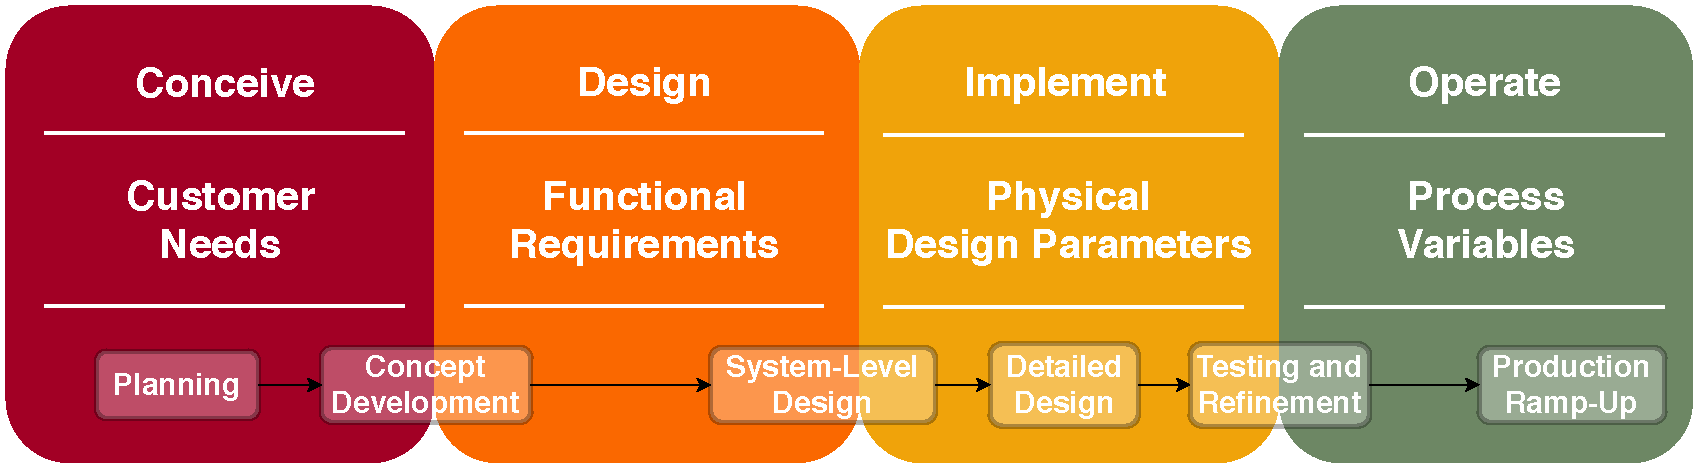
\includegraphics[width=0.8\textwidth]{design-commonalities}
  \caption[Design]{Design Commonalities\cite{foley2021dindesign}}\label{fig:ru-logo}
\end{figure}
\begin{table}
  \centering
  \begin{tabular}{ll}\toprule
    $x$& $x^{2}$\\\midrule
    1 &1\\
    2 &4\\
    3 &9\\\bottomrule
  \end{tabular}
  \caption{Table of squared numbers}\label{tab:numbers}
\end{table}
There is an example of how to map design methods in CDIO, Axiomatic Design, and Product Design in Figure~\ref{fig:ru-logo}.
This image will scale according to the width of the text on the page.
There is a helpful list of squared numbers in Table~\ref{tab:numbers}.
This table is formatted in the style of a book, which is very differerent than the style one is used to in Excel.

The test text ``Lorem Ipsum''\index{Lorem Ipsum} is from an ancient text from 45 B.C. \cite{cicero46deFinibus, lipsomwebsite}\\
\lipsum[1-5]
\subsection{Subsection}
\lipsum[6-10]
\subsubsection{SubSubsection} 
\lipsum[11-15]
\section[Section with an extremely long name]{Section with a very very very very very very very very very very very very very very very very very very very very long name}
\lipsum[11-18]

%%% Local Variables:
%%% mode: latex
%%% TeX-master: "main"
%%% End:
%include{} starts a new page
\section{Another Section}
\part{The Second Part} % Parts optional but useful in longer documents

\bibliographystyle{IEEEtran/bibtex/ieeetran}
\bibliography{references}

%% If appendices are needed, uncomment the following line
%% and include the appendices in separate files
\appendix{}%%RUM: "Appendicies (as appropriate)
\chapter{Code}\label{cha:code}
You can put code in your document using the \texttt{listings} package, which is
loaded.  Be aware that the \texttt{listings}
package does not put code in your document if you are in draft mode
unless you give it the \texttt{final} option.

There is an example java (Listing~\ref{src:Data_Bus.java}) and XML
file (Listing~\ref{src:AndroidManifest.xml}). Thanks to the
\texttt{url} package, you can typeset OSX and unix paths like this:
\path{/afs/rnd.ru.is/project/thesis-template}. Windows paths:
\path{C:\windows\temp\ }. Note: The \texttt{menukey} package has
similar functionality but may cause problems.

If you are trying to include multiple different languages, you should
go read the documentation and set these up as below.  You
will save yourself a lot of effort, especially if you have to fix
anything.

%% This default style make long lines wrap nicely
\lstdefinestyle{default}{
  %basicstyle=\footnotesize\ttfamily,%
  numbers=left,%
  numberstyle=\tiny,%
  numberfirstline=true,%
  stepnumber=2,%
  numbersep=5pt,%
  columns=fullflexible,%
  tabsize=4,%
  frame=lines,%
  breaklines=true,% break long lines
  prebreak=\raisebox{0ex}[0ex][0ex]{\ensuremath{\color{red}\hookleftarrow}}, % red arrow
  postbreak=\raisebox{0ex}[0ex][0ex]{\ensuremath{\color{red}\hookrightarrow}}, % red arrow
  % from http://tex.stackexchange.com/questions/116534/lstlisting-line-wrapping
}
\lstset{%
  language=,%default similar to verbatim
  style=default,
}

%% The pre-defined languages we want to use.
\lstloadlanguages{Java, XML}

%% We can also define a new language (so we can change some formatting)
%% Be careful you do not make a recursive style nor language!!
%% You can just use the XML language, or in this case create a "dialect"
\lstdefinelanguage[android]{XML}%
{  % 
  sensitive=false,% case-insensitive
  classoffset=0,  % first class
  morekeywords={manifest},
  classoffset=1,  % second class
  morekeywords={uses, sdk, application, activity},
  keywordstyle=\color{blue}, % set a color
  classoffset=0, % reset back to 0
}

%% We use listing styles to adjust the appearance
%% Be careful you do not make a recursive style nor language!!
%% This makes use of the listing package to show program output
\lstdefinestyle{progoutput}{
  language=sh, 
  frame=single, 
  breaklines=true,
  prebreak=\textbackslash,
  captionpos=b,   
  basicstyle=\small\ttfamily, 
  showstringspaces=false 
}

%%I have put the source code in the \directory{src/} folder.
\lstinputlisting[language=Java, firstline=1,
lastline=40, caption={Data\_Bus.java: Setting up the class.},
label={src:Data_Bus.java}]{src/Data_Bus.java}

\lstinputlisting[language={[android]XML}, firstline=1, lastline=20,
caption={AndroidManifest.xml: Configuration for the Android UI.},
label={src:AndroidManifest.xml}]{src/AndroidManifest.xml}

%% TODO: fix wrapping from custom.sty

%%% Local Variables:
%%% mode: latex
%%% TeX-master: "main"
%%% TeX-engine: luatex
%%% End:
 % as an example, perhaps some of your code

%\backmatter{} % Sections after this don't get numbers
%% We prefer that all elements be numbered

%%%%%%%%%%%%% SHOW INDEX %%%%%%%%%%%%%%%%%%
%% Index, optional.  A good idea on longer documents
\clearforchapter{}
\printindex{}%%RUM: Not mentioned

\end{document}
%%% Local Variables:
%%% mode: latex
%%% TeX-master: t
%%% End:
